\documentclass[aspectratio=169]{beamer}
\useoutertheme[progressbar=frametitle]{metropolis}
\useinnertheme{metropolis}
\definecolor{nabgray}{rgb}{0.6,0.59,0.61}
\usecolortheme[named=nabgray]{structure}
\usepackage{tikz}
\usepackage[utf8]{inputenc}
\usepackage[spanish]{babel}
\usepackage{fontspec}
\setmonofont{JetBrains Mono}
\setmainfont{Roboto}
\setsansfont{Roboto}
\usepackage{hyperref}
\usepackage{smartdiagram}
\usepackage{qtree}
\usepackage{verbatim}
\usepackage{svg}
\usepackage{graphicx}
\usepackage{color}
\definecolor{lightgray}{rgb}{0.95, 0.95, 0.95}
\definecolor{darkgray}{rgb}{0.4, 0.4, 0.4}
\definecolor{ocherCode}{rgb}{1, 0.5, 0} % #FF7F00 -> rgb(239, 169, 0)
\definecolor{blueCode}{rgb}{0, 0, 0.93} % #0000EE -> rgb(0, 0, 238)
\definecolor{greenCode}{rgb}{0, 0.6, 0} % #009900 -> rgb(0, 153, 0) 

\usepackage{upquote}
\usepackage{listings}
\lstset{language=java,
    otherkeywords={var,record,permits},
	% Basic design
	backgroundcolor=\color{lightgray},
	basicstyle={\small\ttfamily},   
	frame=l,
	keywordstyle=\footnotesize\color{blue},
	escapeinside={<@}{@>},
	breaklines=true,
	% Line numbers
	xleftmargin={0.75cm},
	numbers=left,
	stepnumber=1,
	firstnumber=1,
	numberfirstline=true
	% Code design
	identifierstyle=\color{black},
	keywordstyle=\color{ocherCode}\bfseries,
	ndkeywordstyle=\color{greenCode}\bfseries,
	stringstyle=\color{ocherCode}\ttfamily,
	commentstyle=\color{darkgray}\ttfamily,
	tabsize=2,
	showtabs=true,
	showspaces=false,
	showstringspaces=false,
	extendedchars=true,
	breaklines=true
}

\lstdefinelanguage{bash}{
    basicstyle=\ttfamily,
    showstringspaces=false,
    commentstyle=\color{red},
    keywordstyle=\color{blue},
    numbers=right,
    xleftmargin={0.25cm}
}

\usebackgroundtemplate
{
	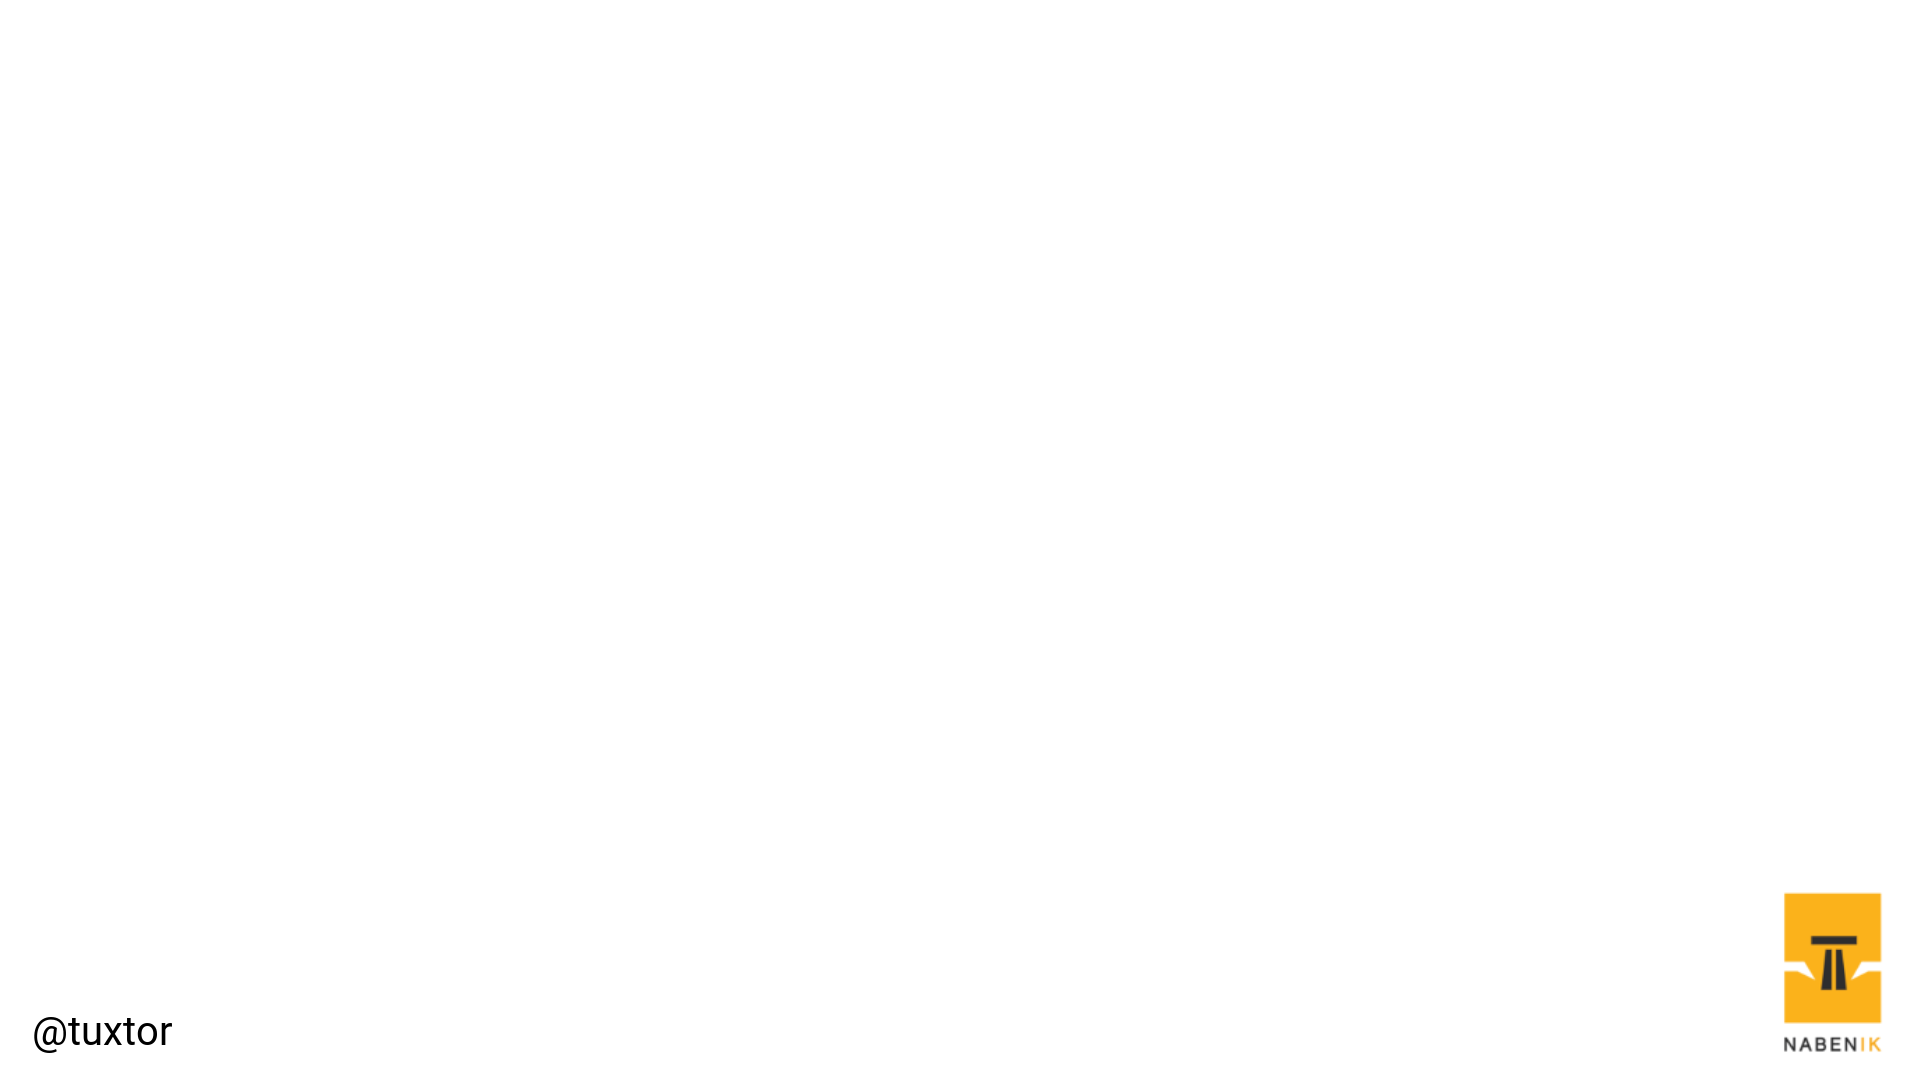
\includegraphics[width=\paperwidth]{Images/fondo}%
}


\title{Desde Java 8 hasta Java 17}
\author{Víctor Orozco - @tuxtor}
\institute{Nabenik}
\date{\today}

\begin{document}

{
    \usebackgroundtemplate{
\includegraphics[width=\paperwidth]{Images/portada}}
    \setbeamercolor{frametitle}{fg=red}
    \usebeamercolor[fg]{normal text}
    \frame{\titlepage}
}


\begin{frame}
    \tableofcontents
\end{frame}


\section{¿Como se hace Java?}

\begin{frame}[fragile]{¿Java?}
	\begin{itemize}
		\item Lenguaje
		\item VM
		\item Bibliotecas/API
	\end{itemize}

El conjunto es la plataforma Java (TM)
	
\end{frame}

\begin{frame}[fragile]{¿Como se actualiza Java?}
	\begin{itemize}
		\item JCP - Java Community Process
		\item JSR - Java Specification Request
		\item JEP - Java Enhancement Proposal
		\item JCK - Java Compatibility Kit
	\end{itemize}	
\end{frame}



\begin{frame}[fragile]{¿Como se actualiza Java? - Java Enhancement Proposal}
	\begin{figure}
		\centering
		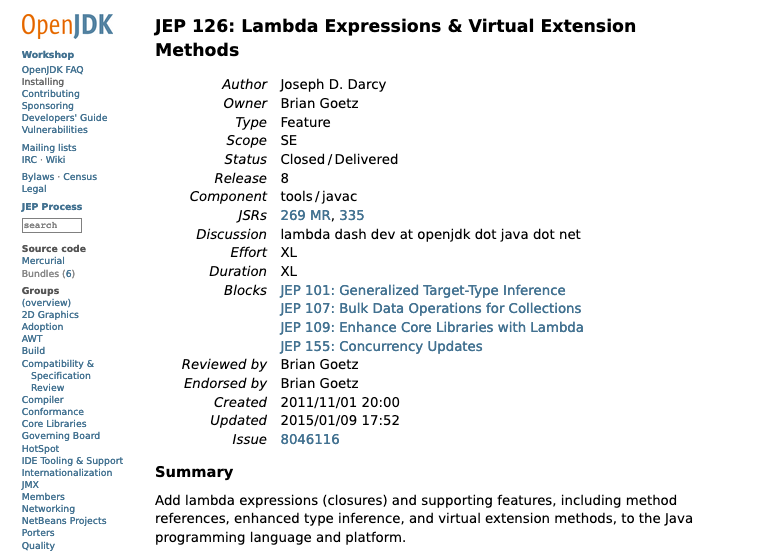
\includegraphics[width=0.9\linewidth]{Images/jep}
	\end{figure}
	
\end{frame}

\begin{frame}[fragile]{¿Como se actualiza Java? - Java Compatibility Kit}
	\begin{figure}
		\centering
		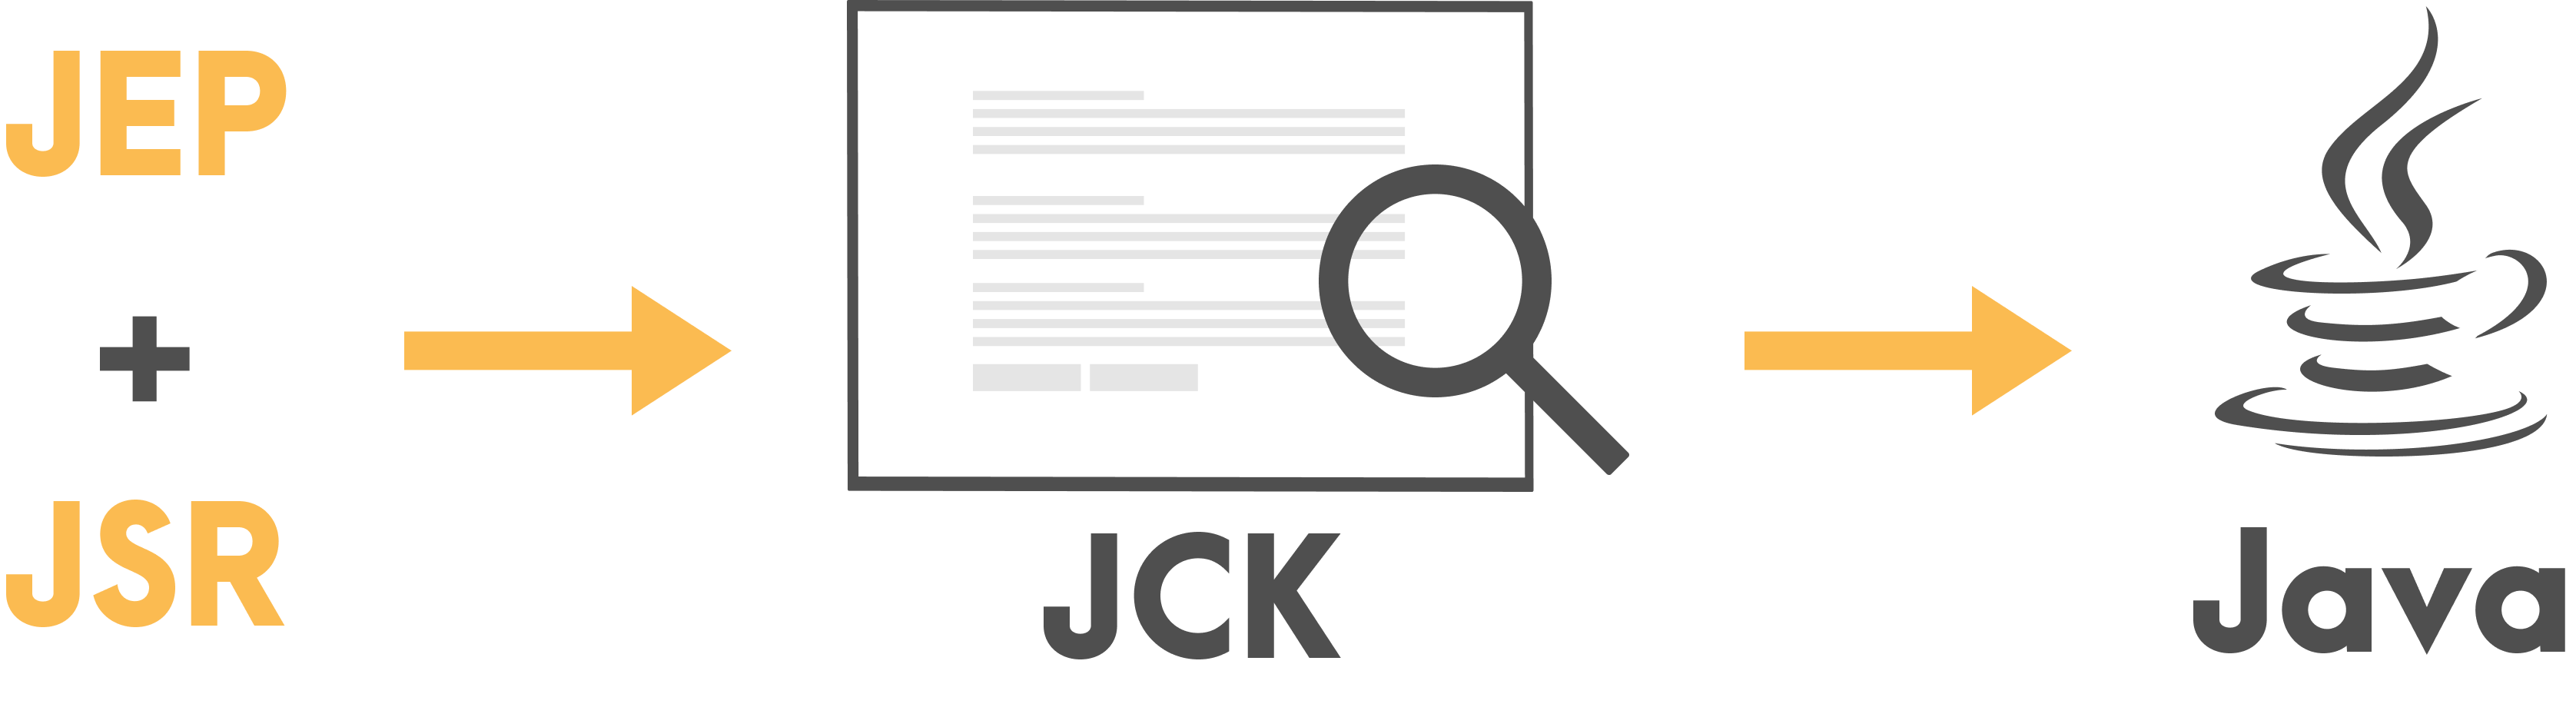
\includegraphics[width=0.9\linewidth]{Images/jck}
	\end{figure}
	
\end{frame}

\begin{frame}[fragile]{Distros}

\begin{figure}
\centering
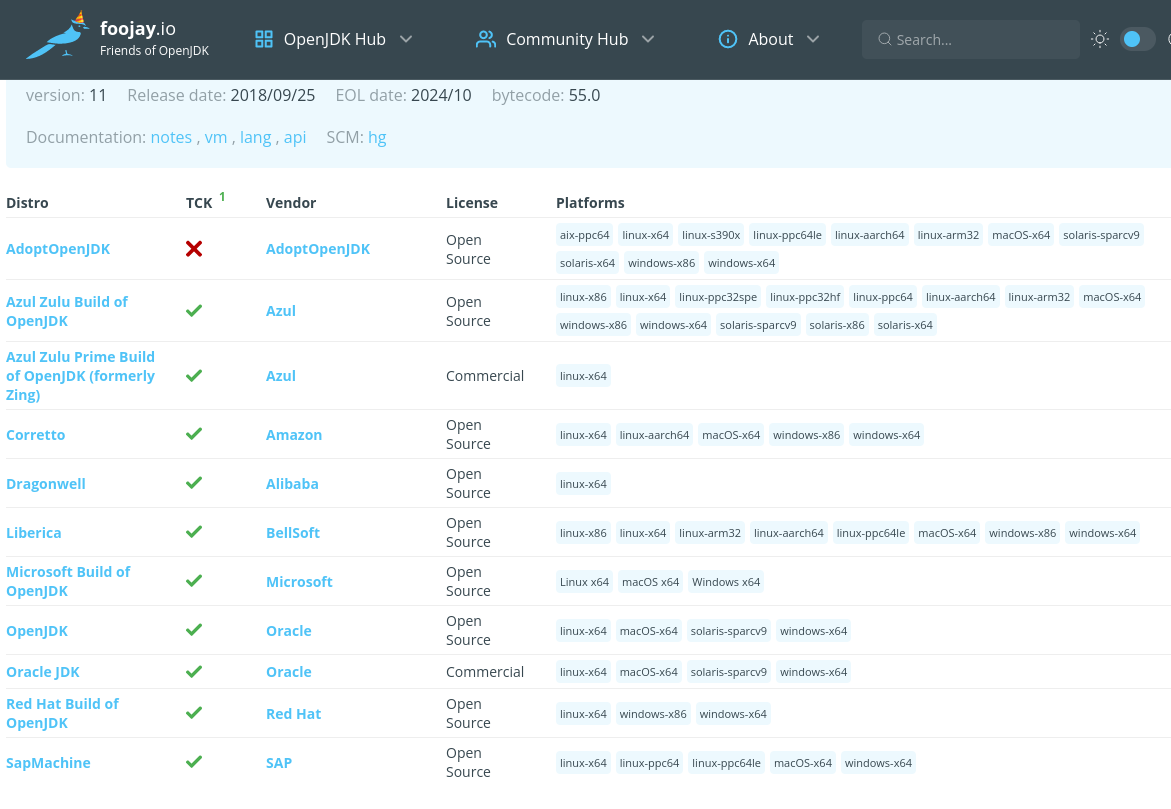
\includegraphics[width=0.7\linewidth]{Images/foojay.png}
\end{figure}


\end{frame}

{
    \usebackgroundtemplate{
\includegraphics[width=\paperwidth]{Images/separador}}
    \setbeamercolor{normal text}{fg=white}
    \setbeamercolor{frametitle}{fg=red}
    \usebeamercolor[fg]{normal text}
    \section{De Java 8 hasta Java 17}
}

\begin{frame}[fragile]{¿Que versión de Java se usa más en Guatemala?}
\LARGE Java 8

\url{https://guatejug.github.io/jvm2021/}
\end{frame}




%TODO Timeline

\begin{frame}[fragile]{¿Que recibo con cada versión nueva de Java?}
	\begin{itemize}
		\item Java - \textbf{Lenguaje}
		\item Java - Bibliotecas e APIs
		\item Java - Maquina Virtual de Java
	\end{itemize}	
    Mejoras de tipo
    \begin{itemize}
   		\item Incubation
   		\item Preview (--flag)
   		\item Definitiva
   	\end{itemize}	
\end{frame}



\begin{frame}[fragile]{Java - Las mejoras que resaltan}
	\begin{columns}[T] % contents are top vertically aligned
		
		\begin{column}[T]{5cm} % alternative top-align that's better for graphics
			\begin{itemize}
				\item Java 9
				\begin{itemize}
					\item Modulos
					\item JShell
					\item HTTP/2
                    \item Factory methods
				\end{itemize}
				\item Java 10
				\begin{itemize}
					\item Type Inference
					\item Class Data Sharing
					\item Time based release
				\end{itemize}
                 \item Java 11
                \begin{itemize}
                    \item String methods
                    \item File methods
                    \item Direct .java execution
                \end{itemize}
			\end{itemize}
		\end{column}
		\begin{column}[T]{5cm} % each column can also be its own environment
			\begin{itemize}
               
				\item Java 12
				\begin{itemize}
					\item Switch expressions
				\end{itemize}
				\item Java 13
				\begin{itemize}
					\item Text blocks
				\end{itemize}
				\item Java 14
				\begin{itemize}
					\item Pattern matching
					\item Records
					\item Helpfull NPE
				\end{itemize}
			\end{itemize}
		\end{column}
	\end{columns}
\end{frame}




\begin{frame}[fragile]{Java - Las mejoras que resaltan}
	\begin{columns}[T] % contents are top vertically aligned
		
		\begin{column}[T]{5cm} % alternative top-align that's better for graphics
			\begin{itemize}
				\item Java 15
				\begin{itemize}
					\item Sealed classes
					\item Nashorn removal
                    \item SPARC/Solaris removal
				\end{itemize}
				\item Java 16
				\begin{itemize}
					\item Vector API (Incubator)
					\item C++ 14
					\item Records
				\end{itemize}
                
			\end{itemize}
		\end{column}
		\begin{column}[T]{5cm} % each column can also be its own environment
			\begin{itemize}
                \item Java 17
                               \begin{itemize}
                                   \item MacOS Metal
                                   \item Strong encapsulation
                                   \item Switch expression + pattern matching
                                   \item AOT removal
                                                                  \item Applet deprecation
                               \end{itemize}
			\end{itemize}
		\end{column}
	\end{columns}
\end{frame}


{
    \usebackgroundtemplate{
\includegraphics[width=\paperwidth]{Images/separador}}
    \setbeamercolor{normal text}{fg=white}
    \setbeamercolor{frametitle}{fg=red}
    \usebeamercolor[fg]{normal text}
    \section{Java 9}
}



\begin{frame}[fragile]{JEP 222: jshell: The Java Shell (Read-Eval-Print Loop)}
    \begin{figure}
        \centering
        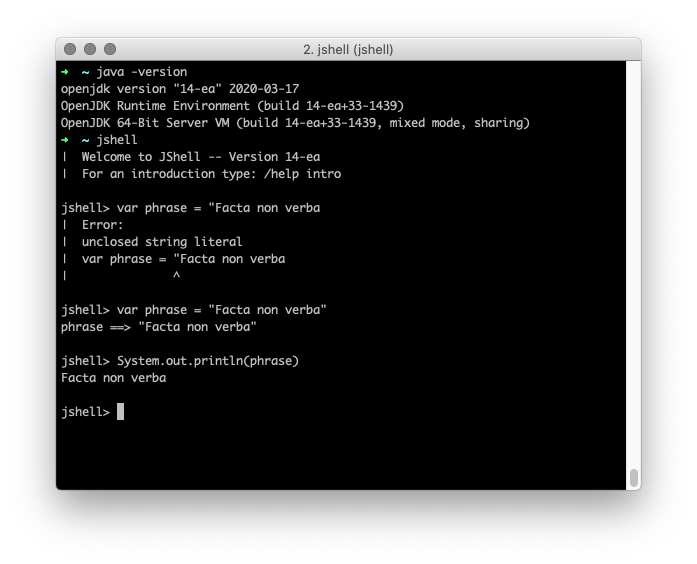
\includegraphics[width=0.9\linewidth]{Images/jshell}
    \end{figure}
    
\end{frame}

\begin{frame}[fragile]{JEP 110: HTTP/2 Client }
\begin{lstlisting}
HttpRequest request = HttpRequest.newBuilder()
    .uri(new URI("https://swapi.co/api/starships/9"))
    .GET()
    .build();

HttpResponse<String> response = HttpClient.newHttpClient()
    .send(request, BodyHandlers.ofString());
    
System.out.println(response.body());
\end{lstlisting}
\end{frame}


\begin{frame}[fragile]{JEP 269: Convenience Factory Methods for Collections}
Antes
\begin{lstlisting}
Set<String> set = new HashSet<>();
set.add("a");
set.add("b");
set.add("c");
set = Collections.unmodifiableSet(set);
\end{lstlisting}	

"Pro"
\begin{lstlisting}
Set<String> set = Collections.unmodifiableSet(new HashSet<>(Arrays.asList("a", "b", "c")));
\end{lstlisting}	

Ahora
\begin{lstlisting}
Set<String> set = Set.of("a", "b", "c");
\end{lstlisting}
\end{frame}


\begin{frame}[fragile]{JEP 213: Milling Project Coin - Private methods in interfaces}
Antes
\begin{lstlisting}
public interface Vehicle{
    public void move();
}
\end{lstlisting}	

Ahora
\begin{lstlisting}[basicstyle=\scriptsize\ttfamily]
public interface Vehicle{
    public default void makeNoise(){
        System.out.println("Making noise!");
        createNoise();
    }

    private void createNoise(){
        System.out.println("Run run");
    } 
}
\end{lstlisting}	
    
\end{frame}

\begin{frame}[fragile]{JEP 213: Milling Project Coin - Try-with-resources}
Antes
\begin{lstlisting}
BufferedReader reader = new BufferedReader(new FileReader("langs.txt"));

try(BufferedReader innerReader = reader){
    System.out.println(reader.readLine());
}
\end{lstlisting}	

Ahora
\begin{lstlisting}
BufferedReader reader = new BufferedReader(new FileReader("langs.txt"));

try(reader){
    System.out.println(reader.readLine());
}
\end{lstlisting}	
    
\end{frame}

{
    \usebackgroundtemplate{
\includegraphics[width=\paperwidth]{Images/separador}}
    \setbeamercolor{normal text}{fg=white}
    \setbeamercolor{frametitle}{fg=red}
    \usebeamercolor[fg]{normal text}
    \section{Java 10}
}


\begin{frame}[fragile]{Java 10}
\textbf{286: Local-Variable Type Inference}\\
296: Consolidate the JDK Forest into a Single Repository\\
304: Garbage-Collector Interface\\
307: Parallel Full GC for G1\\
\textbf{310: Application Class-Data Sharing}\\
312: Thread-Local Handshakes\\
313: Remove the Native-Header Generation Tool (javah)\\
314: Additional Unicode Language-Tag Extensions\\
316: Heap Allocation on Alternative Memory Devices\\
317: Experimental Java-Based JIT Compiler\\
319: Root Certificates\\
\textbf{322: Time-Based Release Versioning}\\
\end{frame}

\begin{frame}[fragile]{JEP 286: Local-Variable Type Inference}
\begin{lstlisting}
public static void main(String args[]){
    var localValue = 99;
    System.out.println(++localValue);
    //localValue = "Foo"
}
\end{lstlisting}	
\end{frame}



\begin{frame}[fragile]{JEP 310: Application Class-Data Sharing}
\begin{lstlisting}[language=bash,basicstyle=\scriptsize]
java -XX:+UseAppCDS -XX:DumpLoadedClassList=classes.lst -jar demo-microservicio-ee-microbundle.jar
java -XX:+UseAppCDS -Xshare:dump -XX:SharedClassListFile=classes.lst -XX:SharedArchiveFile=app-cds.jsa demo-microservicio-ee-microbundle.jar
java -XX:+UseAppCDS -Xshare:on -XX:SharedArchiveFile=app-cds.jsa -jar demo-microservicio-ee-microbundle.jar
\end{lstlisting}	
\end{frame}
\begin{frame}[fragile]{JEP 310: Application Class-Data Sharing}
    \begin{figure}
        \centering
        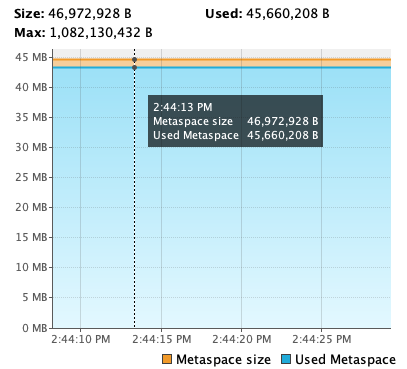
\includegraphics[width=0.7\linewidth]{Images/nocdsmem}
    \end{figure}
\end{frame}
\begin{frame}[fragile]{JEP 310: Application Class-Data Sharing}
    \begin{figure}
        \centering
        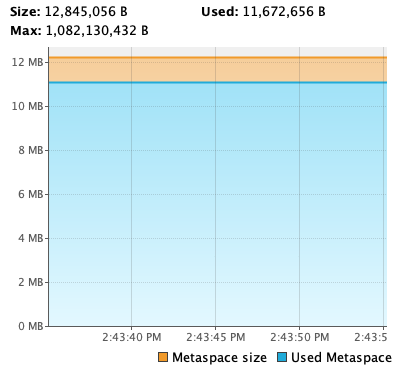
\includegraphics[width=0.7\linewidth]{Images/cdsmem}
    \end{figure}
\end{frame}


\begin{frame}[fragile]{JEP 322: Time-Based Release Versioning}
    \begin{figure}
        \centering
        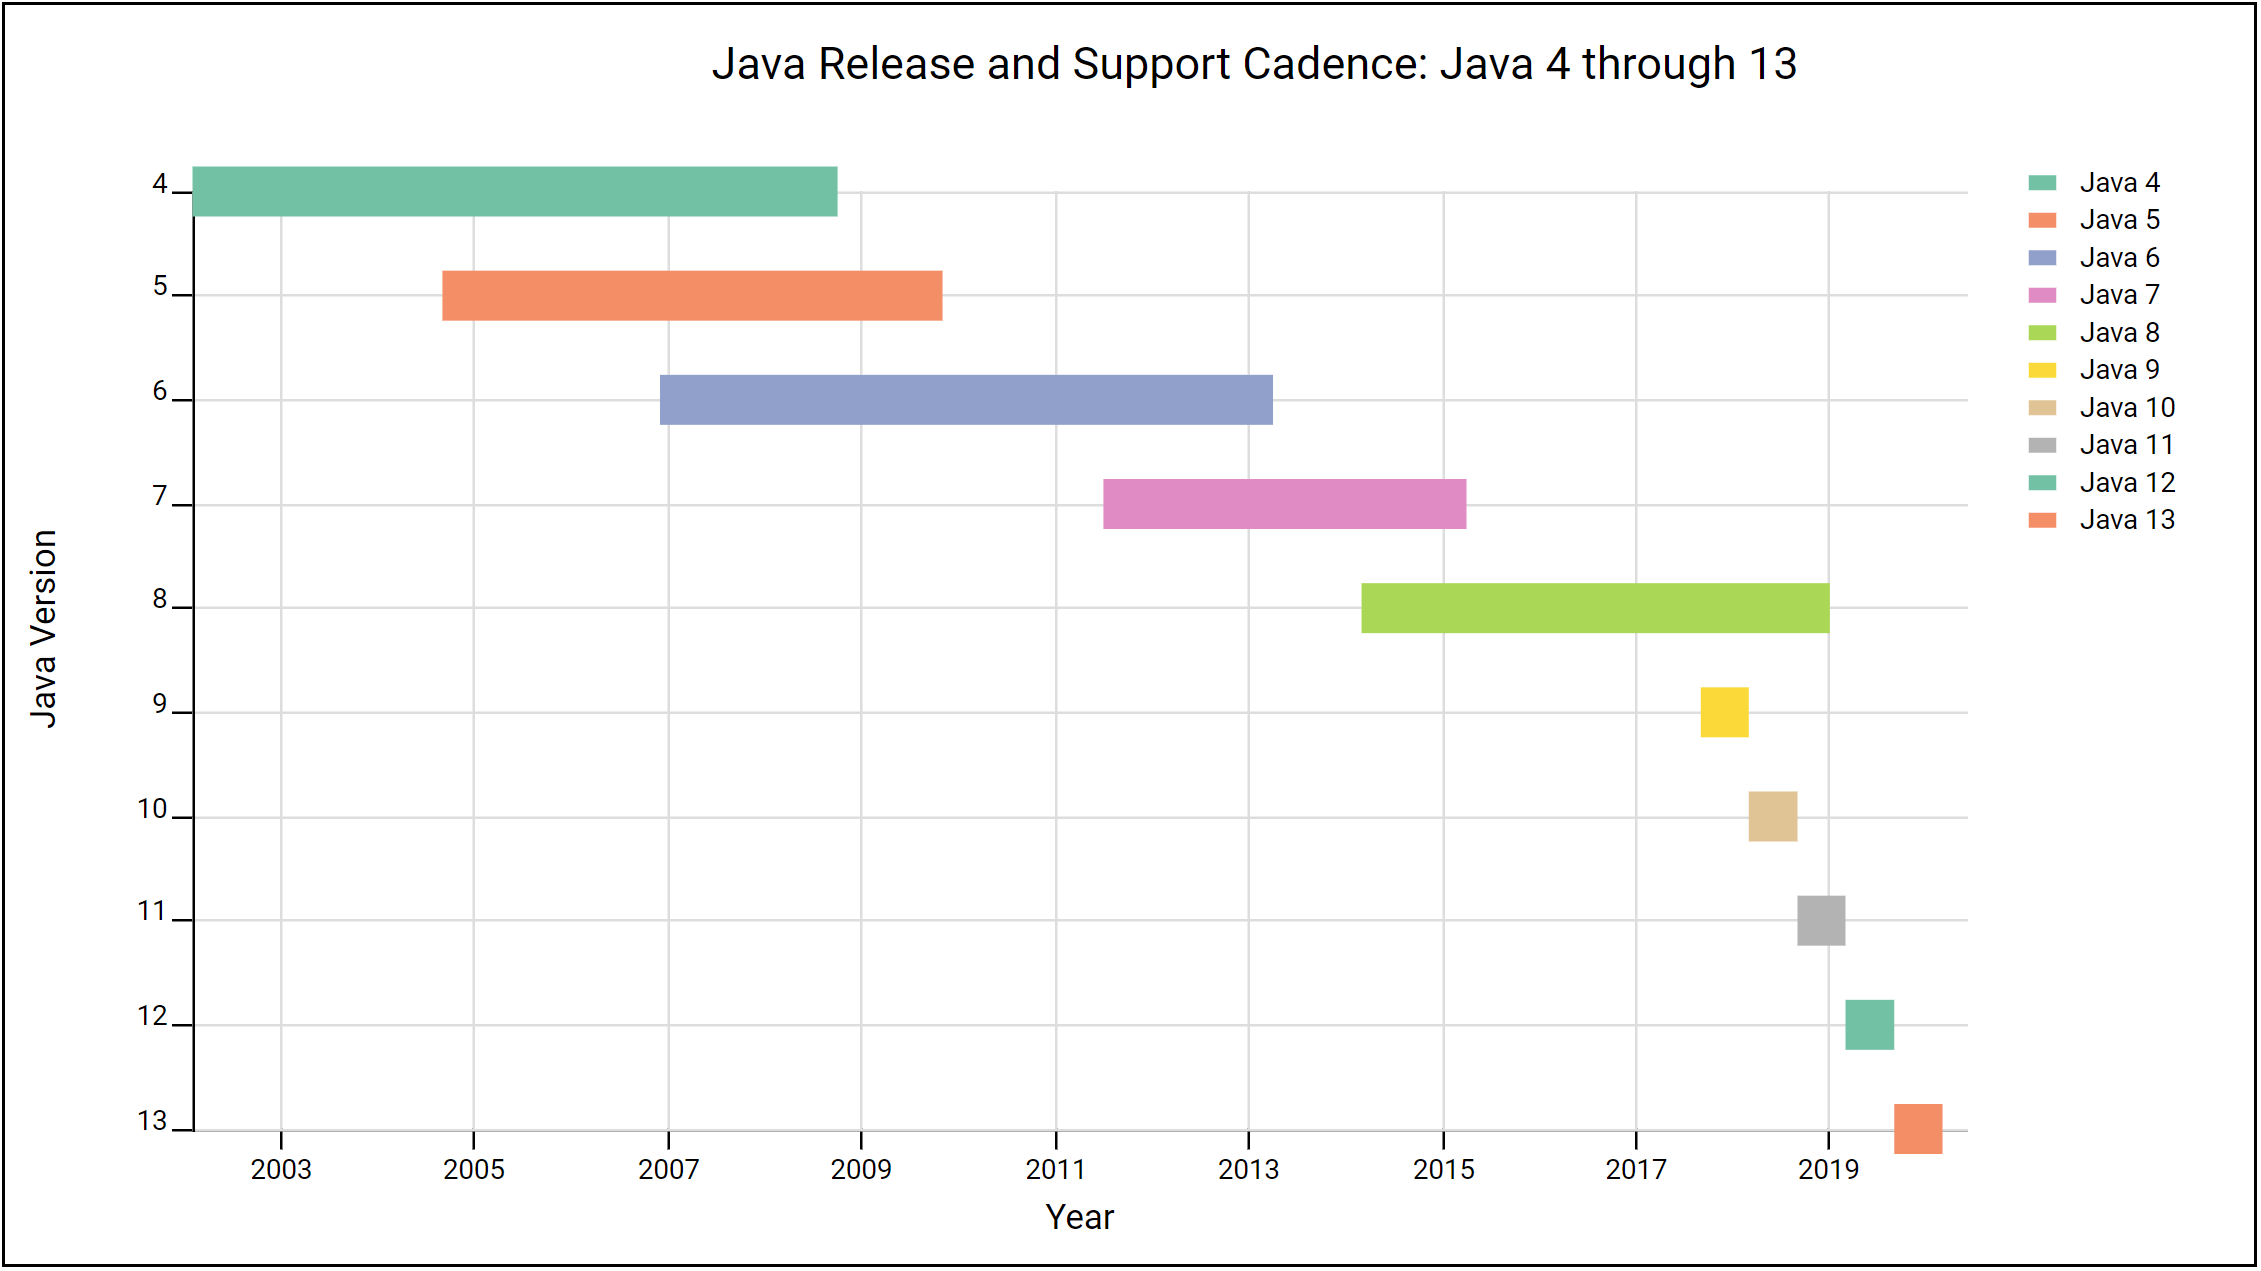
\includegraphics[width=0.9\linewidth]{Images/javacadence}
    \end{figure}
\end{frame}
   
\begin{frame}[fragile]{JEP 322: Time-Based Release Versioning}
    \begin{figure}
        \centering
        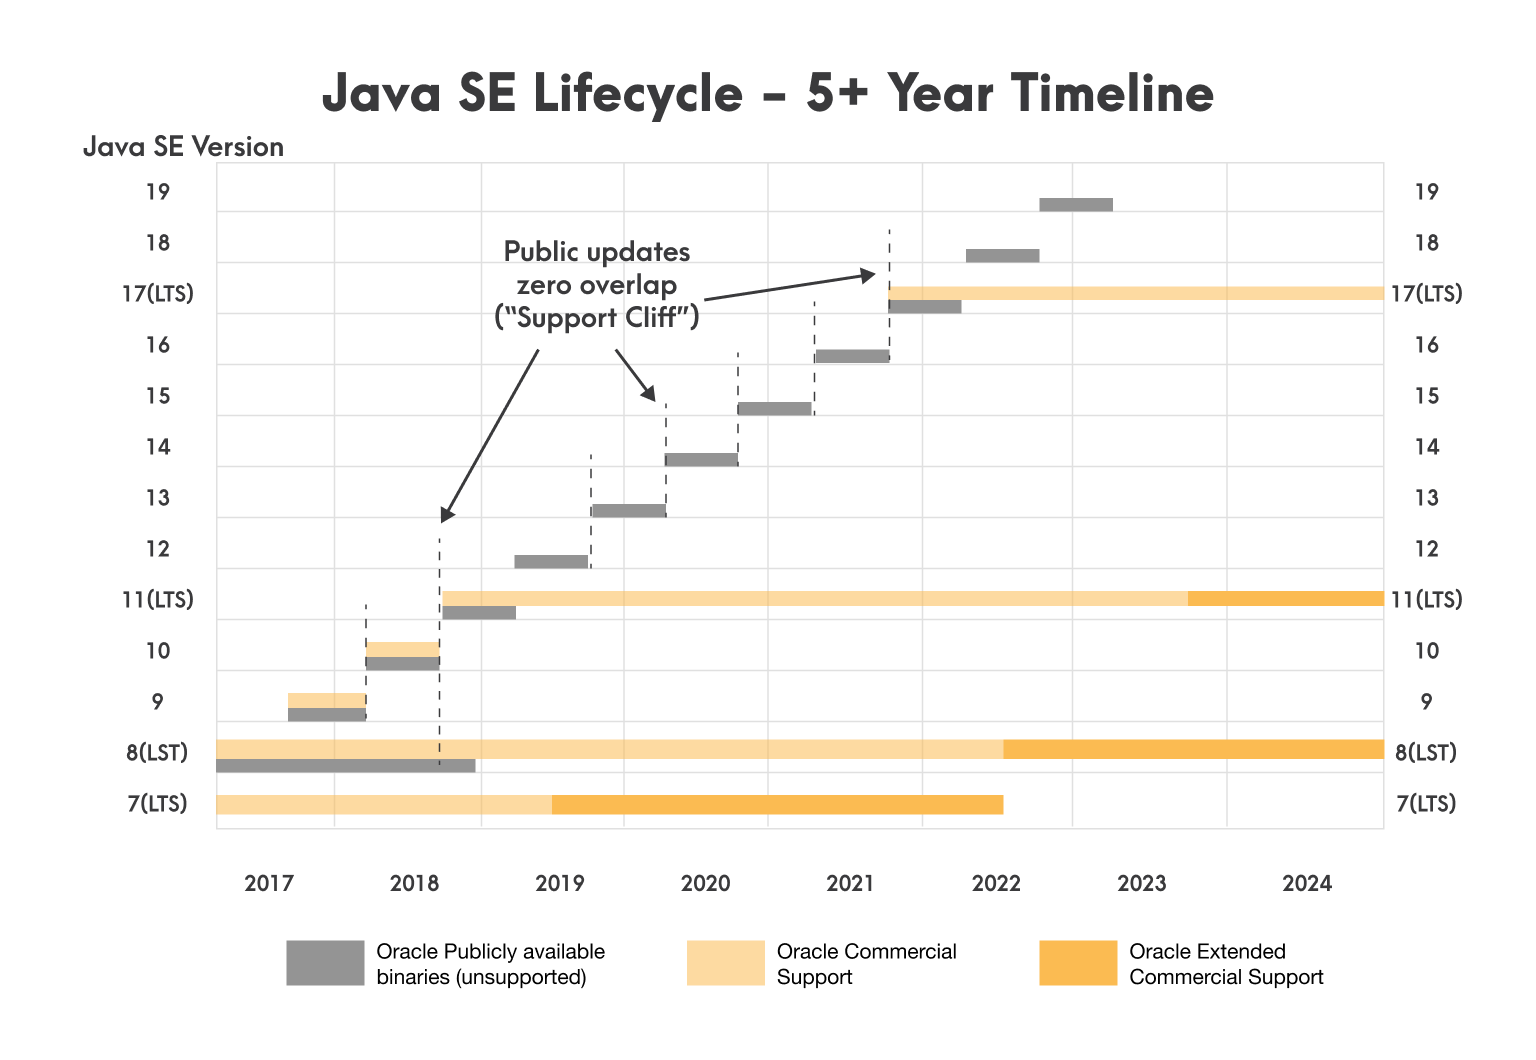
\includegraphics[width=0.9\linewidth]{Images/javarelease}
    \end{figure}
\end{frame}

{
    \usebackgroundtemplate{
\includegraphics[width=\paperwidth]{Images/separador}}
    \setbeamercolor{normal text}{fg=white}
    \setbeamercolor{frametitle}{fg=red}
    \usebeamercolor[fg]{normal text}
    \section{Java 11}
}

\begin{frame}[fragile]{Java 11}\scriptsize
\begin{columns}[T] % contents are top vertically aligned
    
    \begin{column}[T]{6cm} % alternative top-align that's better for graphics
        181: Nest-Based Access Control\\
        309: Dynamic Class-File Constants\\
        315: Improve Aarch64 Intrinsics\\
        318: Epsilon: A No-Op Garbage Collector\\
        \textbf{320: Remove the Java EE and CORBA Modules}\\
        321: HTTP Client (Standard)\\
        \textbf{323: Local-Variable Syntax for Lambda Parameters}\\
        324: Key Agreement with Curve25519 and Curve448\\
        327: Unicode 10\\
        328: Flight Recorder\\
    \end{column}
    \begin{column}[T]{6cm} % each column can also be its own environment
        329: ChaCha20 and Poly1305 Cryptographic Algorithms\\
        \textbf{330: Launch Single-File Source-Code Programs}\\
        331: Low-Overhead Heap Profiling\\
        332: Transport Layer Security (TLS) 1.3\\
        333: ZGC: A Scalable Low-Latency Garbage Collector
        (Experimental)\\
        \textbf{335: Deprecate the Nashorn JavaScript Engine}\\
        336: Deprecate the Pack200 Tools and API\\
    \end{column}
\end{columns}
\end{frame}
    

\begin{frame}[fragile]{JEP 323: Local-Variable Syntax for Lambda Parameters}
Antes
\begin{lstlisting}
BiPredicate<String,String> demoPredicate =
    (String a, String b) -> a.equals(b);
BiPredicate<String,String> demoPredicate =
    (a, b) -> a.equals(b);
\end{lstlisting}

Ahora
\begin{lstlisting}
BiPredicate<String,String> demoPredicate =
    (var a, var b) -> a.equals(b);
\end{lstlisting}	

Posibilidades
\begin{lstlisting}
(@Nonnull var x, @Nullable var y) -> x.process(y)
\end{lstlisting}	
\end{frame}

\begin{frame}[fragile]{JEP 330: Launch Single-File Source-Code Programs}
    \begin{figure}
        \centering
        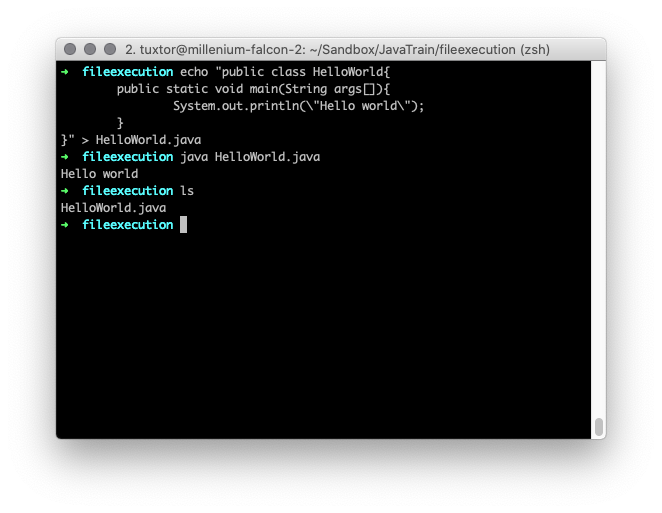
\includegraphics[width=0.9\linewidth]{Images/jep222singlefile}
    \end{figure}
    
\end{frame}

{
    \usebackgroundtemplate{
\includegraphics[width=\paperwidth]{Images/separador}}
    \setbeamercolor{normal text}{fg=white}
    \setbeamercolor{frametitle}{fg=red}
    \usebeamercolor[fg]{normal text}
    \section{Java 12}
}



\begin{frame}[fragile]{Java 12}
189: Shenandoah: A Low-Pause-Time Garbage Collector (Experimental)\\
230: Microbenchmark Suite\\
\textbf{325: Switch Expressions (Preview)}\\
334: JVM Constants API\\
340: One AArch64 Port, Not Two\\
341: Default CDS Archives\\
344: Abortable Mixed Collections for G1\\
346: Promptly Return Unused Committed Memory from G1
\end{frame}


\begin{frame}[fragile]{325: Switch Expressions (Preview)}
Antes
\begin{lstlisting}
String langType = "";
switch (args[0]) {
    case "Java":
    case "Scala":
    case "Kotlin":
        langType = "Static typed";
        break;
    case "Groovy":
    case "JavaScript":
        langType = "Dynamic typed";
        break;
}
System.out.println(langType);
\end{lstlisting}	
\end{frame}

\begin{frame}[fragile]{325: Switch Expressions (Preview)}
Ahora
\begin{lstlisting}
String langType = switch (args[0]) {
    case "Java", "Scala", "Kotlin" -> "Static typed";
    case "Groovy", "JavaScript" -> "Dynamic typed";
    default -> {
        System.out.println("This meant to be a processing block");
        yield "Probably LISP :)";
    }
};
System.out.println(langType);
\end{lstlisting}	
\end{frame}

{
    \usebackgroundtemplate{
\includegraphics[width=\paperwidth]{Images/separador}}
    \setbeamercolor{normal text}{fg=white}
    \setbeamercolor{frametitle}{fg=red}
    \usebeamercolor[fg]{normal text}
    \section{Java 13}
}

\begin{frame}[fragile]{Java 13}
350: Dynamic CDS Archives\\
351: ZGC: Uncommit Unused Memory\\
353: Reimplement the Legacy Socket API\\
354: \textbf{Switch Expressions (Preview)}\\
355: \textbf{Text Blocks (Preview)}\\
\end{frame}

\begin{frame}[fragile]{355: Text Blocks (Preview)}
Antes
\begin{lstlisting}
String html = "<html>\n" +
"    <body>\n" +
"        <p>Hello, world</p>\n" +
"    </body>\n" +
"</html>\n";
\end{lstlisting}

Ahora
\begin{lstlisting}
String html = """
<html>
    <body>
        <p>Hello, world</p>
    </body>
</html>
""";
\end{lstlisting}
\end{frame}

{
    \usebackgroundtemplate{
\includegraphics[width=\paperwidth]{Images/separador}}
    \setbeamercolor{normal text}{fg=white}
    \setbeamercolor{frametitle}{fg=red}
    \usebeamercolor[fg]{normal text}
    \section{Java 14}
}
\begin{frame}[fragile]{Java 14}\scriptsize
    \begin{columns}[T] % contents are top vertically aligned
        
        \begin{column}[T]{6cm} % alternative top-align that's better for graphics
            \textbf{305: Pattern Matching for instanceof (Preview)}\\
            343: Packaging Tool (Incubator)\\
            345: NUMA-Aware Memory Allocation for G1\\
            349: JFR Event Streaming\\
            352: Non-Volatile Mapped Byte Buffers\\
            \textbf{358: Helpful NullPointerExceptions}\\
            \textbf{359: Records (Preview)}\\
            \textbf{361: Switch Expressions (Standard)}
        \end{column}
        \begin{column}[T]{6cm} % each column can also be its own environment
            362: Deprecate the Solaris and SPARC Ports\\
            363: Remove the Concurrent Mark Sweep (CMS) Garbage Collector\\
            364: ZGC on macOS\\
            365: ZGC on Windows\\
            366: Deprecate the ParallelScavenge + SerialOld GC Combination\\
            367: Remove the Pack200 Tools and API\\
            368: Text Blocks (Second Preview)\\
            370: Foreign-Memory Access API (Incubator)
        \end{column}
    \end{columns}
\end{frame}

\begin{frame}[fragile]{JEP 359: Records (Preview)}
Data carrier
\begin{lstlisting}
record Person(String name, String email, int age) {}
\end{lstlisting}

Uso
\begin{lstlisting}
Person foo = new Person("Marco", "example@mail.com",99);
System.out.println(foo);
//foo.name = "Polo";
\end{lstlisting}	
\end{frame}

\begin{frame}[fragile]{305:	Pattern Matching for instanceof (Preview)}
Antes
\begin{lstlisting}
if(o instanceof Person){
    Person p = (Person)o;
    System.out.println("Hello " + p.name());
}else{
    System.out.println("Unknown object");
}
\end{lstlisting}	

Ahora
\begin{lstlisting}
if(o instanceof Person p){
    System.out.println("Hello " + p.name());
}else{
    System.out.println("Unknown object");
}
\end{lstlisting}	
\end{frame}

{
    \usebackgroundtemplate{
\includegraphics[width=\paperwidth]{Images/separador}}
    \setbeamercolor{normal text}{fg=white}
    \setbeamercolor{frametitle}{fg=red}
    \usebeamercolor[fg]{normal text}
    \section{Java 15}
}
\begin{frame}[fragile]{Java 15}\scriptsize
    \begin{columns}[T] % contents are top vertically aligned
        
        \begin{column}[T]{6cm} % alternative top-align that's better for graphics
            339: Addition of EdDSA (Edwards-Curve Digital Signature Algorithm)\\
            \textbf{360: Preview for sealed classes}\\
           \textbf{371: Addition of hidden classes in Java}\\
            372: Removal of the Nashorn JavaScript Engine\\
            373: Legacy DatagramSocket API reimplementation\\
            374: Biased locking disablement and deprecation\\
            375: Second preview for instanceof pattern matching\\
            377: Addition of ZGC, the scalable, low-latency, garbage collector for Java\\
            378: Full inclusion of Java Text Blocks
        \end{column}
        \begin{column}[T]{6cm} % each column can also be its own environment
            379: Addition and enhancements of the low-pause time Shenandoah garbage collector\\
           \textbf{381: Final remove of Solaris and SPARC Ports}\\
            \textbf{383: Incubation of the Foreign-Memory Access API}\\
            384: Second preview inclusion of Java Records\\
            385: RMI Activation deprecation with the goal of future removal
        \end{column}
    \end{columns}
\end{frame}

\begin{frame}[fragile]{360:	Sealed Classes (Preview)}
Antes
\begin{lstlisting}
public class Animal { ... }

public class Porsche extends Animal { ... }
\end{lstlisting}	

Ahora
\begin{lstlisting}
public abstract sealed class Animal
    permits Dog, Cat, Wolf { ... }
\end{lstlisting}	
\end{frame}

\begin{frame}[fragile]{360:	Sealed Classes (Preview)}
Antes
\begin{lstlisting}
public class Animal { ... }

public class Porsche extends Animal { ... }
\end{lstlisting}	

Pro
\begin{lstlisting}
abstract sealed class Animal {
        final class Dog extends Root { ... }
        final class Cat extends Root { ... }
        final class Wolf extends Root { ... }
... }
\end{lstlisting}	
\end{frame}


\begin{frame}[fragile]{371:	Hidden Classes}
Antes
\begin{lstlisting}
ClassLoader::defineClass
\end{lstlisting}	

Ahora
\begin{lstlisting}
Lookup::defineHiddenClass
\end{lstlisting}	
\end{frame}


\begin{frame}[fragile]{381:	Remove the Solaris and SPARC Ports}

\begin{figure}
\centering
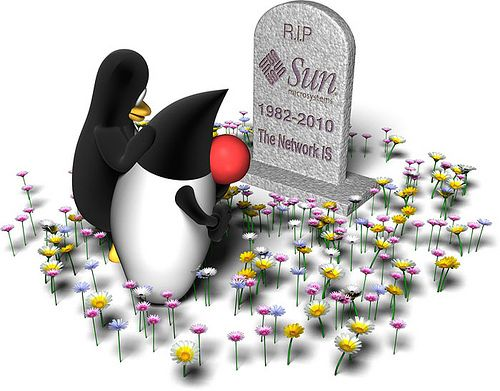
\includegraphics[width=0.7\linewidth]{Images/sun}
\caption{}
\label{fig:sun}
\end{figure}

\end{frame}

\begin{frame}[fragile]{383:	Foreign-Memory Access API (Second Incubator)}

\begin{lstlisting}
VarHandle intHandle = MemoryHandles.varHandle(int.class,
        ByteOrder.nativeOrder());

try (MemorySegment segment = MemorySegment.allocateNative(100)) {
    for (int i = 0; i < 25; i++) {
        intHandle.set(segment, i * 4, i);
    }
    ...
\end{lstlisting}	
\end{frame}


{
    \usebackgroundtemplate{
\includegraphics[width=\paperwidth]{Images/separador}}
    \setbeamercolor{normal text}{fg=white}
    \setbeamercolor{frametitle}{fg=red}
    \usebeamercolor[fg]{normal text}
    \section{Java 16}
}
\begin{frame}[fragile]{Java 16}\scriptsize
    \begin{columns}[T] % contents are top vertically aligned
        
        \begin{column}[T]{6cm} % alternative top-align that's better for graphics
            \textbf{338: Incubation of the Vector API}\\
            347: C++14 language features enablement\\
            357: Migration from Mercurial to Git\\
            369: GitHub migration of OpenJDK repositories\\
            376: Concurrent thread-stack processing for ZGC\\
            380: Unix-Domain Socket Channels\\
            \textbf{386: Alpine Linux port}\\
            387: Support for elastic metaspace\\
            388: The Windows AArch64 Port\\
        \end{column}
        \begin{column}[T]{6cm} % each column can also be its own environment
                389: Incubation of the Foreign Linker API\\
                390: Value-based classes warnings\\
                392: Addition of the Packaging Tool\\
                393: Third incubation of the Foreign-Memory Access API\\
                \textbf{394: Full inclusion of pattern matching for instanceof}\\
                \textbf{395: Full implementation of Java Records}\\
                \textbf{396: Strongly encapsulation of JDK Internals}\\
                397: Second preview of sealed classes
        \end{column}
    \end{columns}
\end{frame}

\begin{frame}[fragile]{386: Alpine Linux Port}

\begin{figure}
\centering

\includegraphics[width=0.7\linewidth]{Images/alpine}
\end{figure}


\end{frame}

\begin{frame}[fragile]{389: Foreign Linker API (Incubator)}


\begin{lstlisting}
LibraryLookup libclang = LibraryLookup.ofLibrary("clang");
LibraryLookup.Symbol clangVersion = libclang.lookup("clang_getClangVersion");
\end{lstlisting}

\end{frame}


\begin{frame}[fragile]{396: Strongly Encapsulate JDK Internals by Default}

Antes
\begin{lstlisting}
--illegal-access=permit 
\end{lstlisting}	

Ahora
\begin{lstlisting}
--illegal-access=deny 
\end{lstlisting}

\end{frame}


{
    \usebackgroundtemplate{
\includegraphics[width=\paperwidth]{Images/separador}}
    \setbeamercolor{normal text}{fg=white}
    \setbeamercolor{frametitle}{fg=red}
    \usebeamercolor[fg]{normal text}
    \section{Java 17}
}
\begin{frame}[fragile]{Java 17}\scriptsize
    \begin{columns}[T] % contents are top vertically aligned
        
        \begin{column}[T]{6cm} % alternative top-align that's better for graphics
            306: Restoration of always-strict semantics for floating-points\\
            356: Pseudo-random number generators improvements\\
            \textbf{382: Support for a new macOS pipeline for rendering}\\
            \textbf{391: The macOS AArch64 port}\\
            \textbf{398: Deprecation of the infamous Applet API with the goal of full removal}\\
            403: Strong encapsulation of Java’s internals\\
            \textbf{406: Switch pattern matching preview}\\
            407: RMI Activation removal\\
        \end{column}
        \begin{column}[T]{6cm} % each column can also be its own environment
             409: Full support for sealed Java classes\\
             410: Removal of the experimental and largely unused ahead-of-time (AOT) and just-in-time (JIT) compilers\\
             411: Deprecation of the Security Manager with removal being the eventual goal\\
             412: Incubation of the Foreign Function \& Memory API\\
             414: Second incubation of the Vector API\\
             415: Context-specific deserialization filters\\
        \end{column}
    \end{columns}
\end{frame}


\begin{frame}[fragile]{406: Pattern Matching for switch (Preview)}

\begin{lstlisting}
static void testTriangle(Shape s) {
    switch (s) {
        case Triangle t && (t.calculateArea() > 100) ->
            System.out.println("Large triangle");
        case Square s ->
            System.out.println("Is not a triangle is a square");
        default ->
            System.out.println("Non-triangle");
    }
}
\end{lstlisting}

\end{frame}
\begin{frame}[fragile]{Nueva licencia Oracle Java 17}

\begin{figure}
\centering
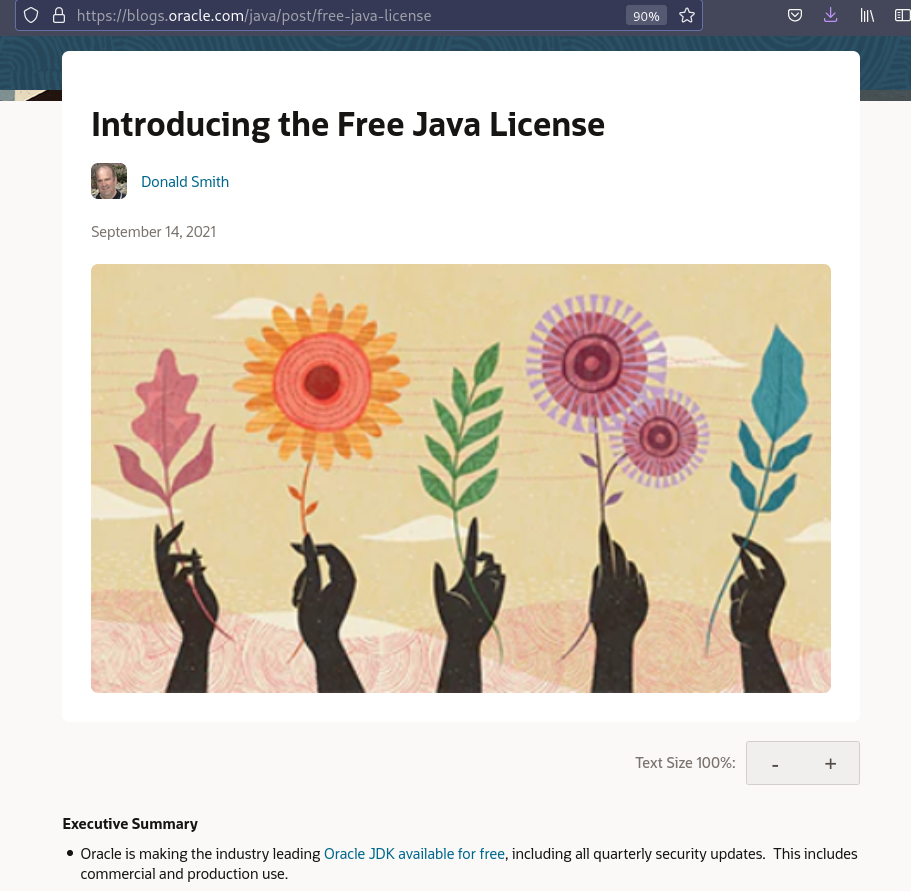
\includegraphics[width=0.7\linewidth]{Images/freejava}
\end{figure}


\end{frame}

\begin{frame}[fragile]{JEPs in JDK 17 integrated since JDK 11}
https://openjdk.java.net/projects/jdk/17/jeps-since-jdk-11
\begin{figure}
\centering
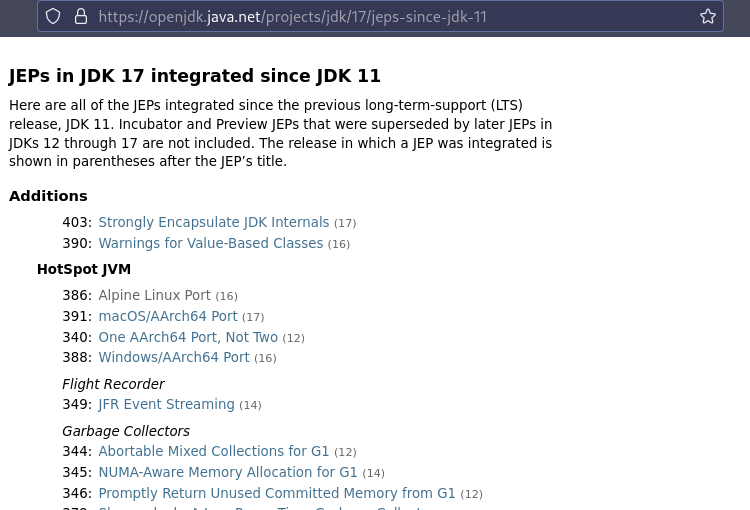
\includegraphics[width=0.7\linewidth]{Images/jepsjava11java17.png}
\end{figure}


\end{frame}




\begin{frame}{Víctor Orozco}
\begin{columns}[T] % contents are top vertically aligned
	
	\begin{column}[T]{4cm} % alternative top-align that's better for graphics
		\begin{figure}
			\centering
			
\includegraphics[width=\linewidth]{Images/logos}
		\end{figure}
	\end{column}
	\begin{column}[T]{6cm} % each column can also be its own environment
		\begin{itemize}
			\item vorozco@nabenik.com
			\item \href{https://twitter.com/tuxtor}{@tuxtor}
			\item \href{http://vorozco.com}{http://vorozco.com}
			\item \href{http://tuxtor.shekalug.org}{http://tuxtor.shekalug.org} 
		\end{itemize}
		\begin{center}
			
\includegraphics[width=0.1\linewidth]{Images/cclogo}
			\\
			This work is licensed under Creative Commons Attribution-NonCommercial-ShareAlike 3.0 Guatemala (CC BY-NC-SA 3.0 GT).
		\end{center}
	\end{column}
\end{columns}
\end{frame}

\end{document}

